% THIS IS AN EXAMPLE DOCUMENT FOR VLDB 2012
% based on ACM SIGPROC-SP.TEX VERSION 2.7
% Modified by  Gerald Weber <gerald@cs.auckland.ac.nz>
% Removed the requirement to include *bbl file in here. (AhmetSacan, Sep2012)
% Fixed the equation on page 3 to prevent line overflow. (AhmetSacan, Sep2012)

\documentclass{vldb}
% \renewcommand{\baselinestretch}{0.99}
\usepackage{graphicx}
\usepackage{balance}  % for  \balance command ON LAST PAGE  (only there!)
\usepackage{enumitem}
\usepackage{hyperref, xcolor}
\hypersetup{colorlinks, citecolor=blue}
     %colorlinks=false,
      %citecolor=Violet,
       %linkcolor=Red,
        %urlcolor=Blue}

\usepackage[T1]{fontenc}
\usepackage[utf8]{inputenc}
\usepackage{authblk}
\usepackage{multirow}
\usepackage{bbding}
\usepackage{pifont}
\usepackage{wasysym}
\usepackage{amssymb}
\usepackage{array,multirow}
\usepackage{cleveref}
\usepackage{soul}

\crefformat{section}{\S#2#1#3} % see manual of cleveref, section 8.2.1
\crefformat{subsection}{\S#2#1#3}
\crefformat{subsubsection}{\S#2#1#3}

\usepackage{url}
\usepackage{balance}

\newcommand\longvar[1]{\mathchardef\UrlBreakPenalty=100
	\mathchardef\UrlBigBreakPenalty=100\url{#1}}

\makeatletter
\newcommand{\printfnsymbol}[1]{%
  \textsuperscript{\@fnsymbol{#1}}%
}
\makeatother

% Include information below and uncomment for camera ready
\vldbTitle{Enabling Data Privacy in Hyperledger Fabric}
\vldbAuthors{}
\vldbDOI{}
\vldbVolume{}
\vldbNumber{}
\vldbYear{}
\balance

\usepackage{nopageno}
% allow hypenation at random places
% but increaces total size of the text
% \sloppy

\begin{document}

% ****************** TITLE ****************************************

\title{Enabling Data Privacy in Hyperledger Fabric\vspace{-.1cm}}
% \author[1]{} %\thanks{contributed equally} } 
% \author[1]{} %\printfnsymbol{1}}
% \author[1]{} % \printfnsymbol{1}}
% \author[2]{}
% \author[1]{}
% \affil[ ]{}
% \affil[ ]{}
%\author{
%	\alignauthor
%	Senthil Nathan\thanks{equally contributed} , Chander Govindarajan\footnotemark[1] , Adarsh Saraf\footnotemark[1] , \\Manish Sethi$^{\$}$, Praveen Jayachandran$^{+}$\\
%	$^{+}$\affaddr{IBM Research, India}\\$^{\$}$\affaddr{IBM RTP, USA}
%	\email{\normalsize{(snatara7, chandg12, adasaraf, praveen.j)@in.ibm.com, manish.sethi1@ibm.com}}
%}
% possible, but not really needed or used for PVLDB:
%\subtitle{[Extended Abstract]
%\titlenote{A full version of this paper is available as\textit{Author's Guide to Preparing ACM SIG Proceedings Using \LaTeX$2_\epsilon$\ and BibTeX} at \texttt{www.acm.org/eaddress.htm}}}

% ****************** AUTHORS **************************************

% You need the command \numberofauthors to handle the 'placement
% and alignment' of the authors beneath the title.
%
% For aesthetic reasons, we recommend 'three authors at a time'
% i.e. three 'name/affiliation blocks' be placed beneath the title.
%
% NOTE: You are NOT restricted in how many 'rows' of
% "name/affiliations" may appear. We just ask that you restrict
% the number of 'columns' to three.
%
% Because of the available 'opening page real-estate'
% we ask you to refrain from putting more than six authors
% (two rows with three columns) beneath the article title.
% More than six makes the first-page appear very cluttered indeed.
%
% Use the \alignauthor commands to handle the names
% and affiliations for an 'aesthetic maximum' of six authors.
% Add names, affiliations, addresses for
% the seventh etc. author(s) as the argument for the
% \additionalauthors command.
% These 'additional authors' will be output/set for you
% without further effort on your part as the last section in
% the body of your article BEFORE References or any Appendices.

%\numberofauthors{4} %  in this sample file, there are a *total*
% of EIGHT authors. SIX appear on the 'first-page' (for formatting
% reasons) and the remaining two appear in the \additionalauthors section.

%\author{
% You can go ahead and credit any number of authors here,
% e.g. one 'row of three' or two rows (consisting of one row of three
% and a second row of one, two or three).
%
% The command \alignauthor (no curly braces needed) should
% precede each author name, affiliation/snail-mail address and
% e-mail address. Additionally, tag each line of
% affiliation/address with \affaddr, and tag the
% e-mail address with \email.
%
% 1st. author
%\alignauthor
%
%Ben Trovato\titlenote{Dr.~Trovato insisted his name be first.}\\
%       \affaddr{Institute for Clarity in Documentation}\\
%       \affaddr{1932 Wallamaloo Lane}\\
%       \affaddr{Wallamaloo, New Zealand}\\
%       \email{trovato@corporation.com}
%% 2nd. author
%\alignauthor
%G.K.M. Tobin\titlenote{The secretary disavows
%any knowledge of this author's actions.}\\
%       \affaddr{Institute for Clarity in Documentation}\\
%       \affaddr{P.O. Box 1212}\\
%       \affaddr{Dublin, Ohio 43017-6221}\\
%       \email{webmaster@marysville-ohio.com}
% 3rd. author
%\alignauthor Lars Th{\Large{\sf{\o}}}rv{$\ddot{\mbox{a}}$}ld\titlenote{This author is the
%one who did all the really hard work.}\\
%       \affaddr{The Th{\large{\sf{\o}}}rv{$\ddot{\mbox{a}}$}ld Group}\\
%       \affaddr{1 Th{\large{\sf{\o}}}rv{$\ddot{\mbox{a}}$}ld Circle}\\
%       \affaddr{Hekla, Iceland}\\
%       \email{larst@affiliation.org}
%\and  % use '\and' if you need 'another row' of author names
%% 4th. author
%\alignauthor Lawrence P. Leipuner\\
%       \affaddr{Brookhaven Laboratories}\\
%       \affaddr{Brookhaven National Lab}\\
%       \affaddr{P.O. Box 5000}\\

%       \email{lleipuner@researchlabs.org}
% There's nothing stopping you putting the seventh, eighth, etc.
% author on the opening page (as the 'third row') but we ask,
% for aesthetic reasons that you place these 'additional authors'
% in the \additional authors block, viz.
% Just remember to make sure that the TOTAL number of authors
% is the number that will appear on the first page PLUS the
% number that will appear in the \additionalauthors section.
%}


\maketitle

\begin{abstract}
	some text \ldots
\end{abstract}


\section{Introduction}
Enterprise blockchain networks are redefining how organizations collaborate on shared data without a central intermediary. In food safety, Walmart demonstrated that a blockchain-based traceability system can reduce the time to trace contaminated produce from seven days to 2.2 seconds~\cite{7-to-2, walmart-hf}. In pharmaceuticals, the MediLedger network~\cite{mediledger} enables drug provenance tracking under the U.S. Drug Supply Chain Security Act, validated through an FDA pilot program. In global trade, GSBN~\cite{gsbn} coordinates private shipping documents across dozens of carriers and ports. In mining, MineHub~\cite{minehub} orchestrates supply-chain workflows across thousands of companies. The common foundation underlying these deployments is a permissioned blockchain: a decentralized, immutable, and transparent ledger that establishes trust among mutually distrusting parties without requiring a central authority.

Yet this very transparency creates a fundamental tension. Enterprise data is inherently private---pricing agreements between a manufacturer and supplier, patient medical records governed by HIPAA~\cite{hipaa-privacy}, identity credentials protected under GDPR~\cite{gdpr}. Storing such data on a fully replicated ledger exposes it to every network participant, including direct competitors. The consequence is stark: organizations must either accept unacceptable privacy violations, or keep private data in siloed off-chain systems, sacrificing the consistency, auditability, and trust guarantees that motivated the blockchain in the first place. This privacy-transparency tradeoff is widely recognized as one of the primary barriers to enterprise blockchain adoption.

Existing approaches are either too coarse-grained, too expensive, or too fragile. \textit{Channels}~\cite{hf}---essentially private sub-networks---provide isolation but require a separate ledger, consensus, and management for each data-sharing relationship, an operational burden that scales poorly as the number of bilateral relationships grows. \textit{Zero-knowledge proofs}~\cite{inproceedings, 7546538} offer strong cryptographic privacy but impose seconds-per-proof computational costs that are prohibitive for high-throughput enterprise workloads. \textit{Trusted Execution Environments}~\cite{ekiden, ccf} rely on specialized hardware and carry well-documented side-channel vulnerabilities. Off-chain databases coupled with on-chain hashes break transactional atomicity: a shipment record and its private invoice cannot be committed atomically across a blockchain and an external store without fragile two-phase commit protocols. None of these approaches simultaneously achieve fine-grained privacy, transactional atomicity, smart-contract integration, and low overhead without specialized hardware (Table~\ref{table:comparison}).
\begin{table}[h]
\centering
\small
\caption{Comparison of Privacy Mechanisms}
\label{table:comparison}
\begin{tabular}{|l|c|c|c|c|}
\hline
\textbf{Mechanism} & \textbf{Fine} & \textbf{Atomic} & \textbf{SC} & \textbf{No HW} \\
 & \textbf{Grained} & & \textbf{Access} & \textbf{Dep.} \\ \hline
Channels & $\times$ & $\checkmark$ & $\checkmark$ & $\checkmark$ \\ \hline
Off-chain DB & $\checkmark$ & $\times$ & $\times$ & $\checkmark$ \\ \hline
ZKPs & $\checkmark$ & $\checkmark$ & Limited\footnotemark & $\checkmark$ \\ \hline
TEEs (e.g., SGX) & $\checkmark$ & $\checkmark$ & $\checkmark$ & $\times$ \\ \hline
\textbf{Pvt. Collections} & $\checkmark$ & $\checkmark$ & $\checkmark$ & $\checkmark$ \\ \hline
\end{tabular}
\vspace{-.3cm}
\end{table}
\footnotetext{ZKP-based smart contracts require expressing all business logic as arithmetic circuits or constraint systems, which limits expressiveness compared to general-purpose languages and imposes significant per-proof computational cost (seconds per proof).}

This paper presents \textit{private data collections} (PDCs), a mechanism that enables fine-grained data privacy within a single blockchain ledger. The key insight is that by storing only the cryptographic hash of private data on the replicated ledger while confining actual data to authorized nodes, the entire network can verify the serializability and integrity of private transactions \textit{without ever seeing the private data itself}---a property we call \textit{blind validation}. Authorized peers process private data in plaintext and simultaneously record its hash on the public ledger; at commit time, any node can validate conflicts by comparing hash versions alone, with no access to the underlying private data required. This eliminates the need for expensive cryptographic primitives or specialized hardware. Unlike channels, PDCs operate within a single ledger; unlike ZKP-based approaches, they impose minimal computational overhead; and unlike off-chain stores, they guarantee transactional atomicity across public and private state. However, because private data is excluded from the consensus-driven block delivery, a critical challenge remains: ensuring that all authorized nodes obtain the private data they need before committing a block. We address this with a gossip-based protocol that proactively disseminates private data during transaction simulation and reactively retrieves missing data before commit, tolerating network partitions and dynamic membership changes.

The main contributions of this paper are as follows:
\begin{itemize}[topsep=0pt,noitemsep,leftmargin=15pt]
    \item We formalize the private data collection abstraction, identify seven design requirements (atomicity, hash-data integrity, smart-contract access control, authorized execution, dynamic membership, data lifecycle management, and data availability), and show that the \textit{execute-order-validate-commit} replication protocol is uniquely suited to support them (\S\ref{pdc}).
    \item We design a dual-layered storage architecture with a \textit{blind validation} mechanism and formally prove that on-chain hashes serve as a conflict-complete proxy for private state, enabling network-wide serializability verification without exposing private data (\S\ref{s:design}).
    \item We propose a two-phase gossip-based protocol combining proactive dissemination with reactive retrieval, supporting dynamic membership changes and tolerating network partitions (\S\ref{s:gossip}).
    \item We implement private data collections in Hyperledger Fabric, an open-source permissioned blockchain platform. The feature has been merged into the Fabric codebase (production-ready since v1.2, with continued enhancements through v2.5) and is deployed in production by organizations including Walmart, MineHub, GSBN, MediLedger, Honeywell, and Oracle.
\end{itemize}

The remainder of this paper is organized as follows. Section~2 motivates the need for data privacy through real-world use cases. Section~3 presents the core idea of our proposed mechanism and analyzes the suitability of different blockchain replication protocols. Section~4 details the design of private data transaction processing. Section~5 describes the data dissemination and retrieval protocol. Section~6 presents the threat model and security analysis. Section~7 discusses implementation. Section~8 presents a performance evaluation. Section~9 describes real-world adoption and impact. Section~10 discusses related work, and Section~11 concludes.


\section{Background and Motivation}
some text \ldots

\subsection{Architecture of Hyperledger Fabric}
some text \ldots

\par
\textbf{(1) Endorsement Phase.} some text \ldots

\par
\textbf{(2) Ordering Phase.} some text \ldots

\par
\textbf{(3) Validation Phase.} some text \ldots

\par
\textbf{(4) Commit Phase.} some text \ldots

\subsection{Motivation for Data Privacy}
\par
some text \ldots
\subsubsection{Use Case Study: Food Traceability}
In September 2006, there was an outbreak of food-borne illness caused by Escherichia coli~\cite{ecoil}
bacteria in 26 U.S. states. This outbreak was linked to bagged spinach. By October 6, 2006, 199 people had been
infected, including three people who died and 31 who suffered kidney failure. It took regulators two
weeks to conduct the backtrace and determine the exact source of the outbreak. During those two weeks,
many people got sick and tons of good spinach was unnecessarily discarded---wrongfully
wasted because we could not tell the good spinach from the bad~\cite{blockchain-for-business}.
An efficient food traceability mechanism is the key to reduce the backtrace time in such a scenario.
Traceability is the ability to track and record the movement of food products throughout a supply chain, which
includes growing, harvesting, packing, manufacturing, repacking, storage, distribution, and sale to the consumer.
With these information, it is possible to trace backward in the supply chain (usually to find the source of a
problem) as well as trace forward (usually to do a recall of contaminated products).
\par
Food Standards Australia New Zealand (FSANZ)~\cite{fs}, European Commission's food safety policy~\cite{eu-foodsafety},
and Food and Agriculture Organization of United Nations (FAO)~\cite{fao-traceability} provide various guidelines on what
records need be kept in order to enable food traceability. The following are some of the records:
\begin{enumerate}[topsep=0pt,noitemsep,leftmargin=15pt]
	\item name and address (and other contact details) of suppliers/farmers and a description of products or inputs supplied.
	\item the name and contact information of the logistics providers and a description of products transpoted.
	\item name and addresses (and other contact details) of customers and a description of the product supplied to them along with the product ID.
    \item date of transaction or delivery.
    \item batch or lot identification (or other markings such as product ID).
    \item volume or quantity of product supplied or received.
	\item raw materials used.
	\item conservation and storage methods for the product.
\end{enumerate}
As a result, when an outbreak of food-borne illness occurrs, it would be possible to traceback from the customer
to the product ID to the supplier/farmer. Similarly, a recall can be performed by tracing forward from the supplier/farmer
to the product lot to customers. If these records are kept in the form of papers or in a centralized database, during
an outbreak, a lot of communication needs to happen between various food business operators to perform traceback
or traceforward. Such a method is very inefficient, time consuming, and expensive.
Hence, a blockchain based food traceability
solution is needed for food safety, to improve efficiency, to allow us to easily communicate information that customers
are asking for (i.e., fork to farm), and to help autheticate claims made in a product. With blockchain, network members
can track the food products as they travel from farm to fork. Recently, Walmart did an experiment that traced
the origin of sliced mangos from Walmart stores back to the farm. This process showed a radical improvement from
approximately seven days it took to conduct the backtrace by using traditional methods down to 2.2
seconds~\cite{7-to-2, walmart-hf} using Hyperledger Fabric.
\par
\begin{figure}
    \begin{center}
	    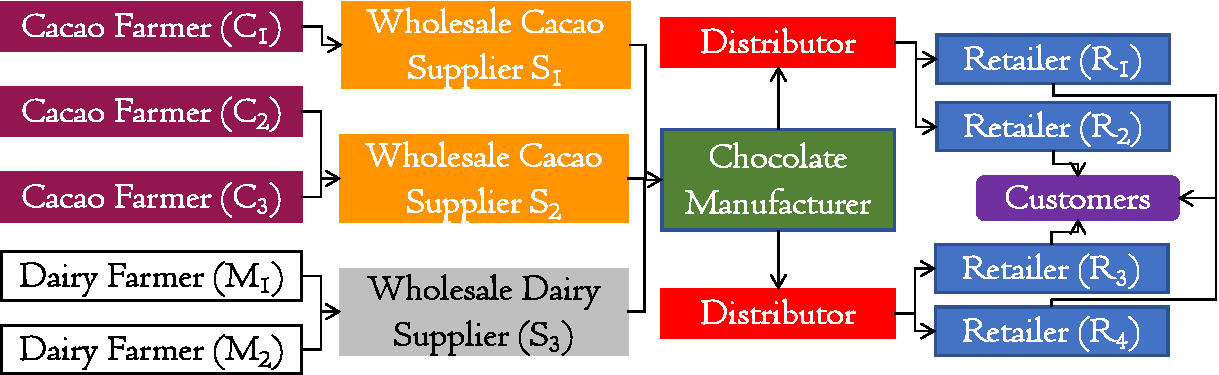
\includegraphics[scale=0.42]{fig/fsc.pdf}
  		\vspace{-.6cm}
		\caption{\small{Actors involved in a simplified food supply chain}.}
	    \label{fig:fsc}
 \end{center}
  \vspace{-.5cm}
\end{figure}
Figure~\ref{fig:fsc} shows actors involved in a simplified chocolate bars supply chain. For manufacturing a
chocolate bar, cacao and milk are required (assume a sugar free chocolate). Usually, manufacturers
buy raw materials from supplier rather than directly contacting various farmers. Once chocolate bars are produced,
via distributors, it would be sent to various retailers across the globe so that the chocolate bars can be sold
to customers. Note that distribution involes import/export authorities, customs and other entities. For simplicity,
we do not cover all involved actors.
\begin{figure}
    \begin{center}
	    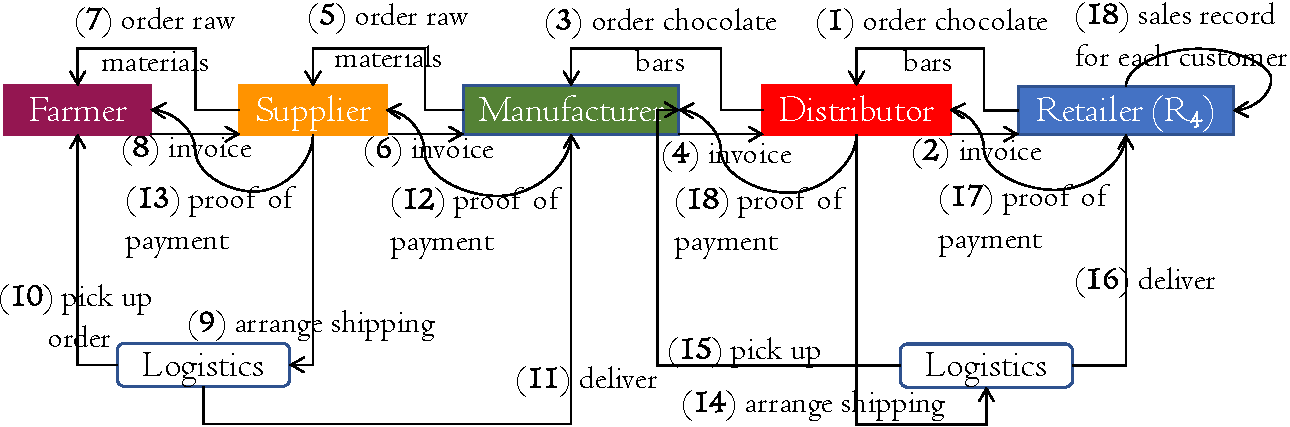
\includegraphics[scale=0.42]{fig/food-supply-chain-tx-flow.pdf}
  		\vspace{-.6cm}
		\caption{\small{A sample transaction flow in a chocolate supply chain}.}
	    \label{fig:tx-flow-fsc}
 \end{center}
  \vspace{-.5cm}
\end{figure}
Figure~\ref{fig:tx-flow-fsc} shows a sample business process in a chocolate supply chain. The process involves
order placement, invoice creation, shipping arrangement, delivery, and proof of payment. The whole process
can be implemented using a permissioned blockchain platform with the help of smart-contracts.
As blockchain is a replicated ledger, storing all information related to above process could leak
proprietary or business competitive information. For example, invoice details cannot be shared as it could leak
the business contract between the farmer and the supplier or the distributor and the retailer. As customer
contact details are very sensitive, it is not advisable to store it in the replicated ledger. However, storing
these details in a blockchain could help in resolving disputes and also it enables a tamper proof record
management for food traceability.
\par
For food traceability, actors don't need to store private/sensitive data in the replicate ledger instead can share information
on demand during an outbreak of food-borne illness. Further, storing the hash of private/sensitive data in the replicated
ledger would help in resolving disputes and tamper proof record management. Assume that a lot of customers are feeling ill due
to a food-borne disease, the food authority needs to find the list of food products each of these customers bought and then
trace it backward in the supply chain to start investigating the root cause. Similarly, it is easy for the actors to trace it
forward to recall potentially contaminated products.
\begin{figure}
    \begin{center}
	    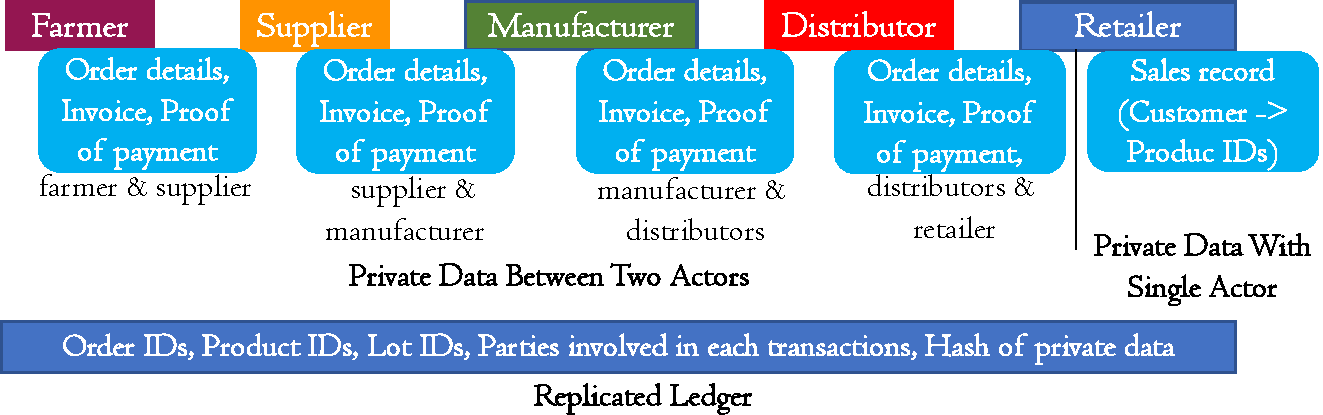
\includegraphics[scale=0.42]{fig/fsc-private-data.pdf}
  		\vspace{-.6cm}
		\caption{\small{Private data should not be shared with all participants as it could leak business contracts or other proprietary information}.}
	    \label{fig:fsc-pvt-data}
 \end{center}
  \vspace{-.5cm}
\end{figure}
\subsubsection{Existing Solutions and Drawbacks}
\par
\textbf{(1) Fabric Channel.}
\par
\textbf{(2) Quorum~\cite{} Private Transaction.}
\par
\textbf{(3) Encryption of Data.}
\par
\textbf{(4) Off-chain Storage With an On-chain Proof.}
\par
\textbf{(5) Zero Knowledge Proof.}


% \section{Design of Public Ledger}
some text \ldots

\subsection{Channels and Pluggable Database Layer}
some text \ldots

\subsection{Transaction Simulation, Validation, and Commit}
some text \ldots

\subsection{Block Storage}
some text \ldots

\subsection{History Database and Provenance Queries}
some text \ldots

\subsection{Failure and Recovery}
some text \ldots

\subsection{Point in Time Rollback}
some text \ldots

\subsection{Backup and Restore}
some text \ldots


\section{Design of Private Ledger}
some text \ldots

\subsection{Private Data Collection}
some text \ldots

\subsection{Transaction Simulation, Validation, and Commit}
some text \ldots

\subsection{Private Data Store}
some text \ldots

\subsection{Missing Private Data, Dynamic Collection, and Reconciliation}
some text \ldots

\subsection{Purging of Expired Private Data}
some text \ldots

\subsection{Failure and Recovery}
some text \ldots

\subsection{Point in Time Rollback}
some text \ldots




% \section{Design of Gossip Protocol}
very tentative. just to put out a layout.

\subsection{Membership Information}
some text \ldots

\subsection{Block Dissemination and Channels}
some text \ldots

\subsection{Private Data Dissemination During Simulation and Commit}
some text \ldots

\subsection{Reconciliation of Missing Private Data}
some text \ldots

\subsection{Block Reprocessing After a Rollback}
some text \ldots


\section{Implementation}
some text \ldots


\section{Evaluation}

\textbf{TODO: Evaluation experiments to include:}
\begin{enumerate}[topsep=0pt,noitemsep,leftmargin=15pt]
    \item Throughput comparison: PDC transactions vs.\ standard transactions
    \item Latency breakdown across the four phases (simulation, ordering, validation, commit)
    \item Scalability with number of collections, organizations, and private data sizes
    \item Gossip overhead: network bandwidth for dissemination and retrieval
    \item Impact of block-to-live (purging) on performance
    \item Comparison with channel-based isolation (the main alternative)
    \item Failure/recovery scenarios and their performance impact
    \item Addition of new members to the collection and sync/fetch duration
\end{enumerate}


\section{Discussion and Future Work}
some text \ldots



\section{Related Work}
\yacov{I'll take this part if you don't mind $:)$}
\textbf{(1) Fabric Channel.}
\par
\textbf{(2) Quorum~\cite{} Private Transaction.}
\par
\textbf{(3) Encryption of Data.}
\par
\textbf{(4) Zero Knowledge Proof.}



\section{Conclusion}

We presented \textit{private data collections} (PDCs): private data is stored only on authorized peers while its cryptographic hash is recorded on the replicated ledger. The key theoretical result is that on-chain hashes form a \textit{conflict-complete proxy} for private state (Theorem~1): optimistic concurrency control (OCC)~\cite{occ} based serializability checks on hashed state detect exactly the same conflicts as checks on the underlying private data, enabling network-wide correctness verification without accessing private data. A transient store, hashed read-write sets, and a three-component dissemination protocol deliver privacy, atomicity, integrity, and auditability within a single shared ledger---without specialized hardware, expensive cryptographic primitives, or channel-based overhead. Our Hyperledger Fabric implementation, production-ready since v1.2, adds 3--14\% overhead. Deployments at Walmart, MediLedger, GSBN, and MineHub confirm cross-industry generality.


% The following two commands are all you need in the
% initial runs of your .tex file to
% produce the bibliography for the citations in your paper.
\bibliographystyle{abbrv}
\bibliography{pvtdata}  % vldb_sample.bib is the name of the Bibliography in this case
% You must have a proper ".bib" file
%  and remember to run:
% latex bibtex latex latex
% to resolve all references

\end{document}
%%% Local Variables:
%%% mode: latex
%%% TeX-master: t
%%% End:
